\renewcommand{\thefigure}{B.\arabic{figure}}
\renewcommand{\thesection}{B.\arabic{section}}
\chapter{Results of Analysis on Low Interference Data}
\section{Tavarola - \textbf{ICB}}
\begin{figure}[h!]
    \centering
    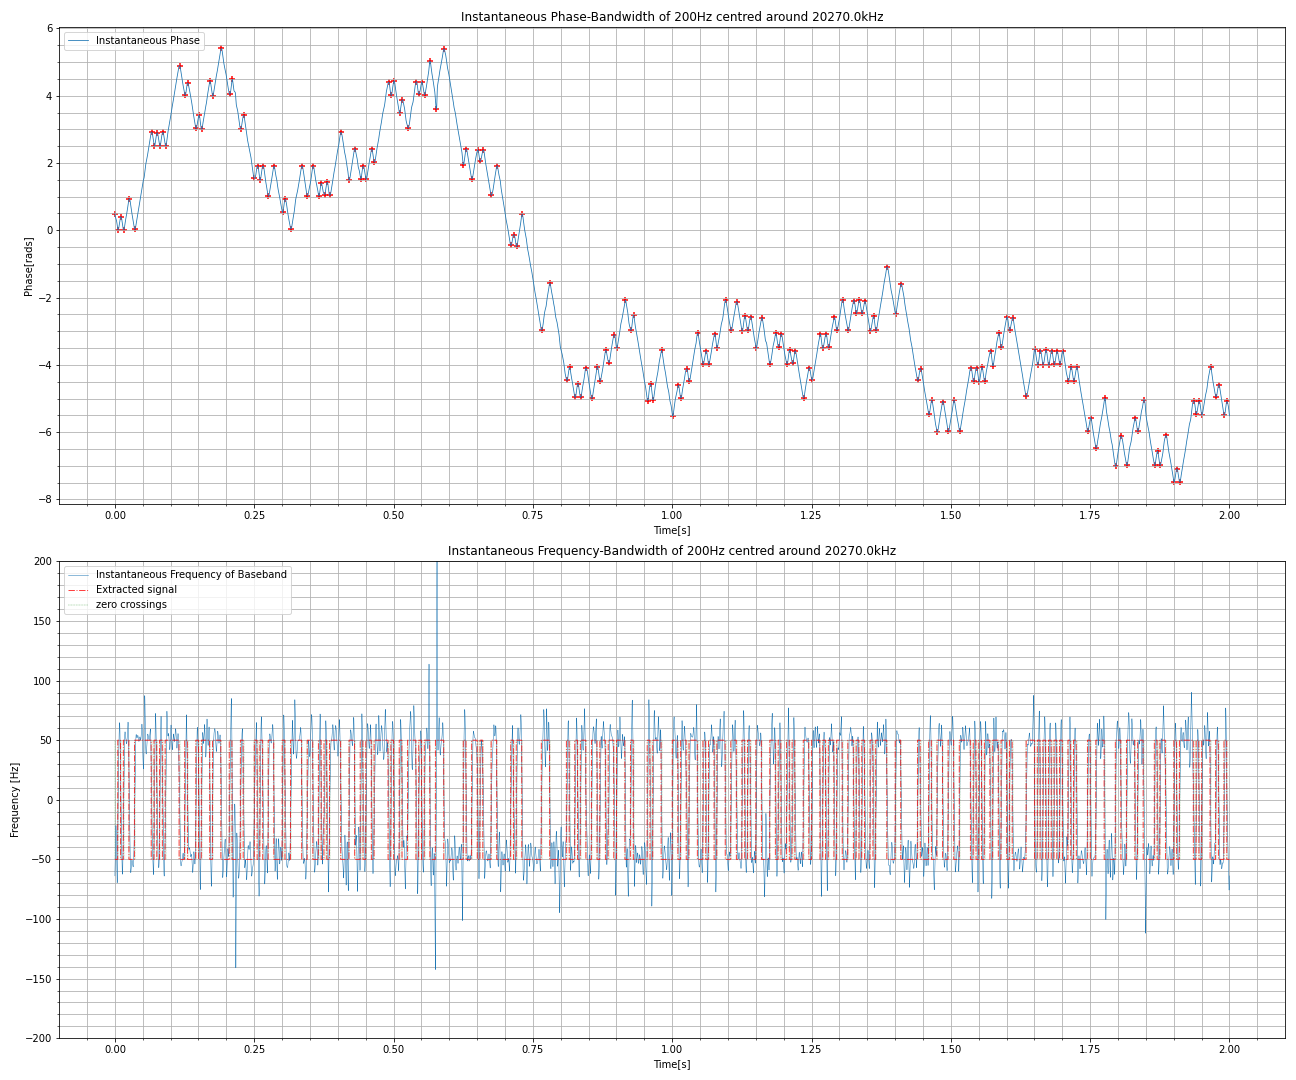
\includegraphics[width = \textwidth]{figs/AppB/ICV.png}
    \caption{Demodulated Signal Transmitter ICV. Instantaneous Phase and Frequency Shown}
    \label{fig:ICV}
\end{figure}
\newpage
\section{Skelton - \textbf{GZQ}}
\begin{figure}[h!]
    \centering
    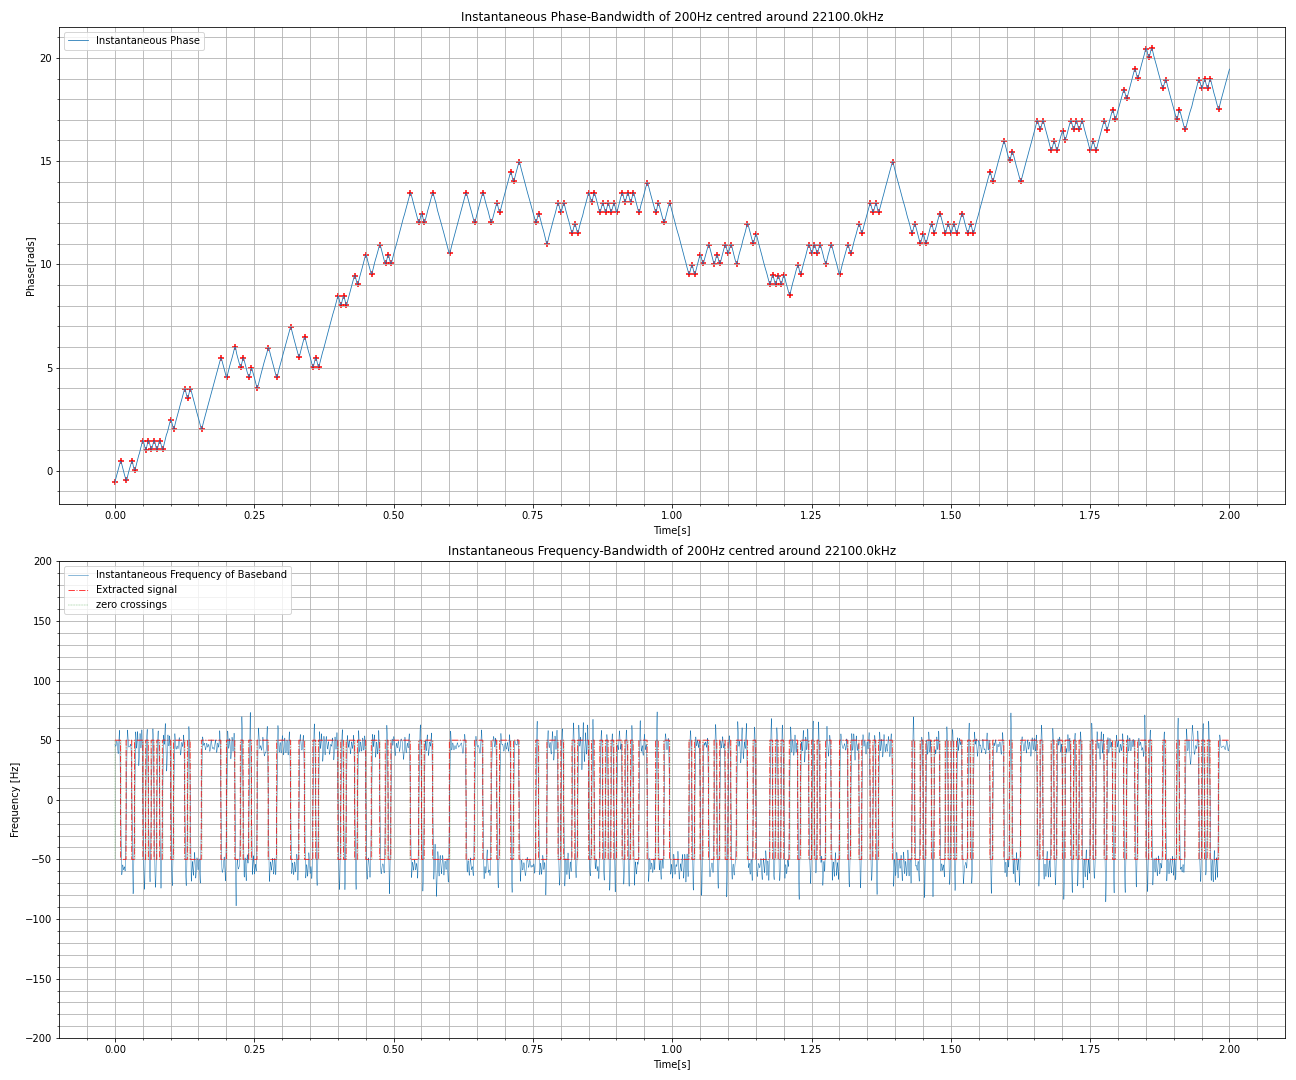
\includegraphics[width = \textwidth]{figs/AppB/GZQ.png}
    \caption{Demodulated Signal Transmitter GZQ. Instantaneous Phase and Frequency Shown}
    \label{fig:GZQ}
\end{figure}
\newpage
\section{Rhauderfehn - \textbf{DHO}}
\begin{figure}[h!]
    \centering
    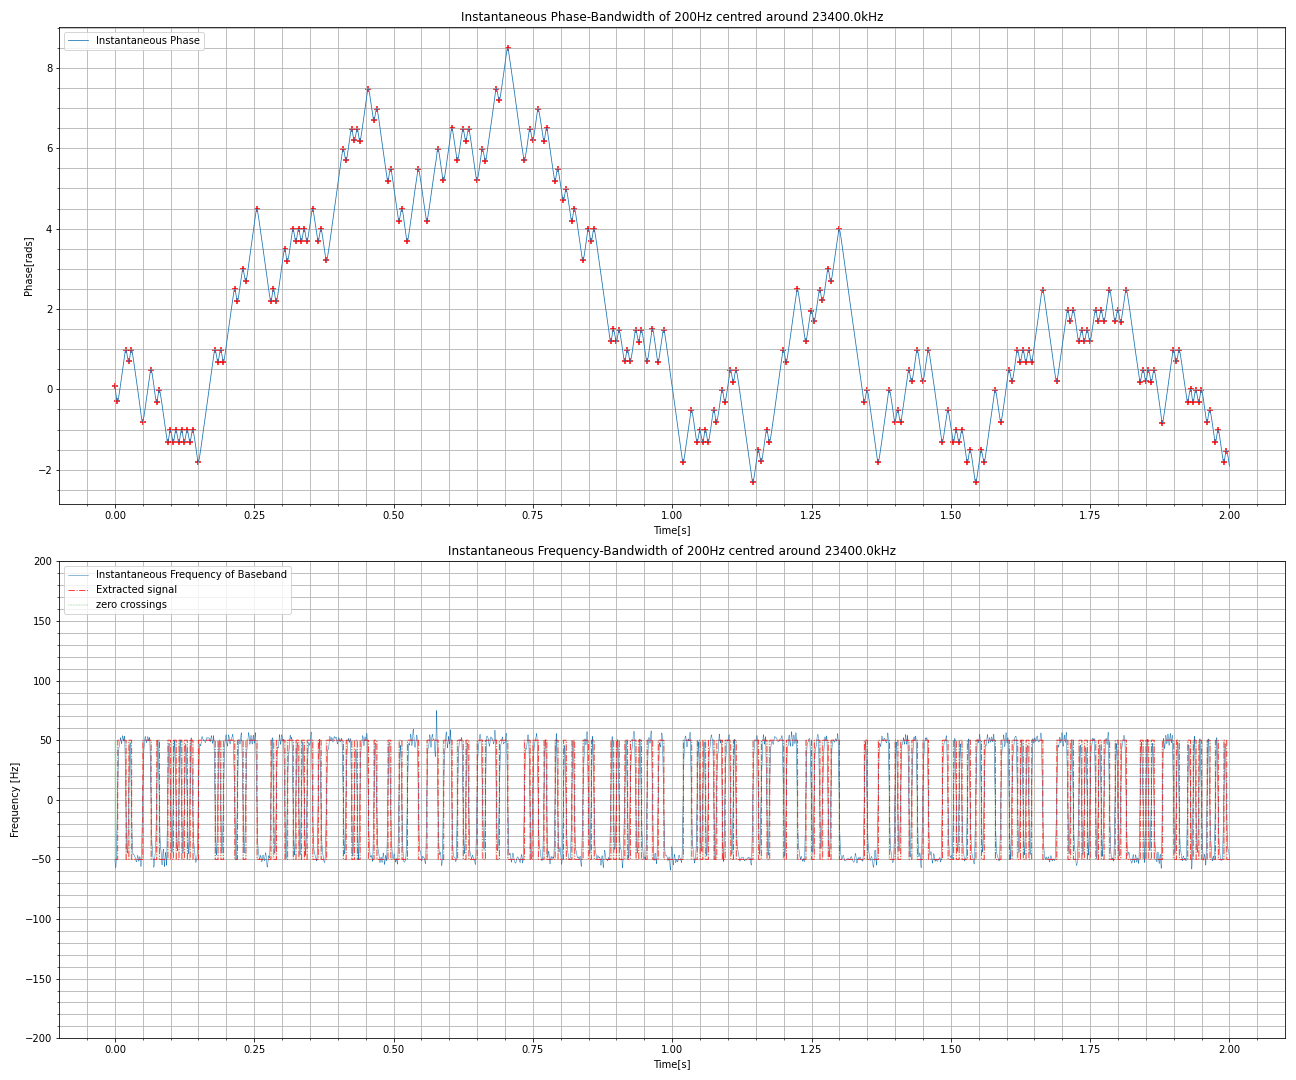
\includegraphics[width = \textwidth]{figs/AppB/DHO.png}
    \caption{Demodulated Signal Transmitter DHO. Instantaneous Phase and Frequency Shown}
    \label{fig:DHO}
\end{figure}
\newpage
\section{Cutler - \textbf{NAA}}
\begin{figure}[h!]
    \centering
    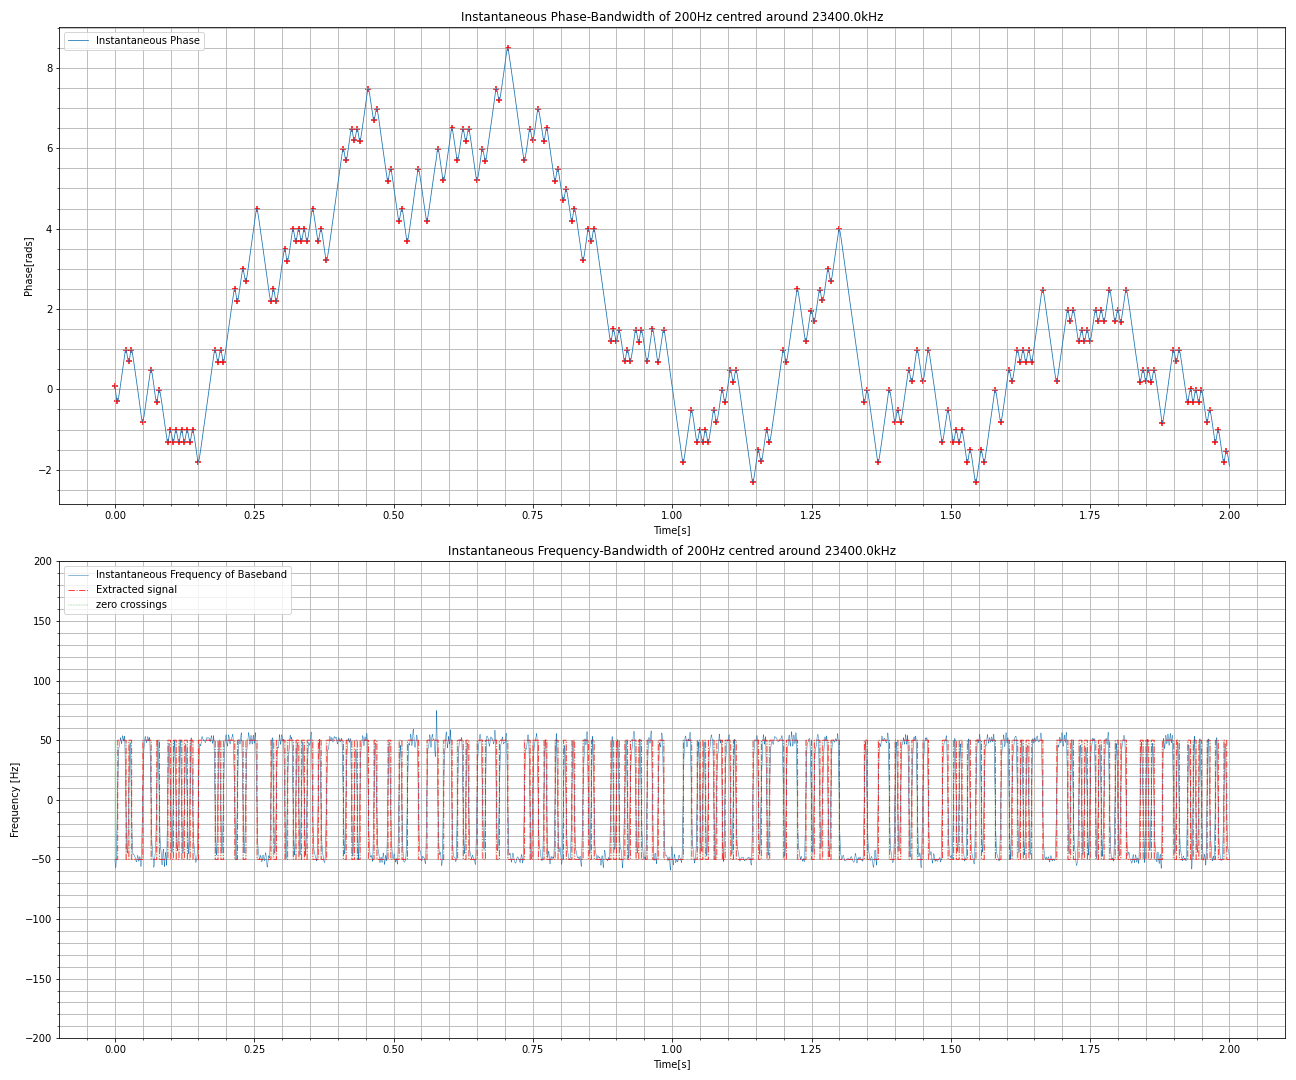
\includegraphics[width = \textwidth]{figs/AppB/NAA.png}
    \caption{Demodulated Signal Transmitter NAA. Instantaneous Phase and Frequency Shown}
    \label{fig:NAA}
\end{figure}